
\status{NUMERICALLY\_VALIDATED}
The Julia input derivative export agrees with centered differences to
$2.16\times10^{-9}$ relative.
The maximum coefficient-check errors are
$3.59\times10^{-6}$ (cubic PLL change)
and $1.85\times10^{-10}$ (integral-gain change).
Arb arithmetic encloses the hidden inverse, a nonzero nine-dimensional gauge
minor, a nonzero residue denominator, and all ten weight signs for the explicitly
gauge-restored binary export. This is not a physical uncertainty certificate.
The fourteen rounded collective designs have interval-enclosed
$|\kappa_3|<10^{-12}$; literal exact neutrality is not attributed to rounded gains.

At the fixed replacement of 87.646222\%, or
4735.315954 MW, changing uniform PLL delay from 40 to 41 ms gives:
\begin{center}
\begin{tabular}{lrr}
\toprule Method & Catalog $\alpha$ (s$^{-1}$) & $\|\Delta K_p/K_p\|_2$\\
\midrule
Unchanged & 0.413952 & 0.000000\\
Sitewise compensation & 0.490670 & 0.031324\\
Moment only & 0.405520 & 0.011050\\
Modal only & -0.060001 & 0.091062\\
Collective moment and modes & -0.058573 & 0.085815\\
\bottomrule
\end{tabular}
\end{center}
The collective candidate's solver status is
\texttt{MAX\_ITERATIONS}; no global optimum is claimed.
It passes the original $-0.05$ guard but misses the auxiliary $-0.0600001$
target. The modal-only candidate reaches that tighter target but its line
search stalls. Their costs do not establish superiority at an equal achieved
modal margin; neither run proves a local optimum.
The complete-region numerical DDE contour gives
\texttt{PASS\_NUMERICAL}.
All 5 of 5 frozen 60 s nonlinear events pass; the
worst excursion is 0.465929Hz and windowed RoCoF is
0.219224Hz/s. Current-limiter safety is not modeled.
The delay-perturbed candidate retains 667.445136 MW of SG;
this experiment does not optimize replacement.

\begin{figure}[htbp]\centering
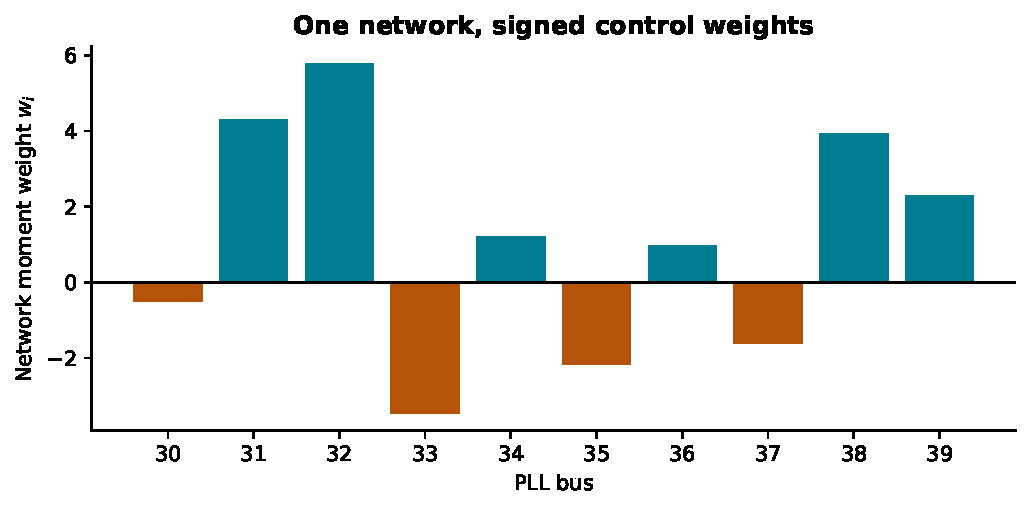
\includegraphics[width=.84\linewidth]{experiments/network_moment_codesign_20261004/FIG_01_NETWORK_WEIGHTS.pdf}
\caption{Network moment weights for the fixed IEEE--39 design. Their signs
are interval-verified for the symmetry-restored exported model.}\end{figure}
\begin{figure}[htbp]\centering
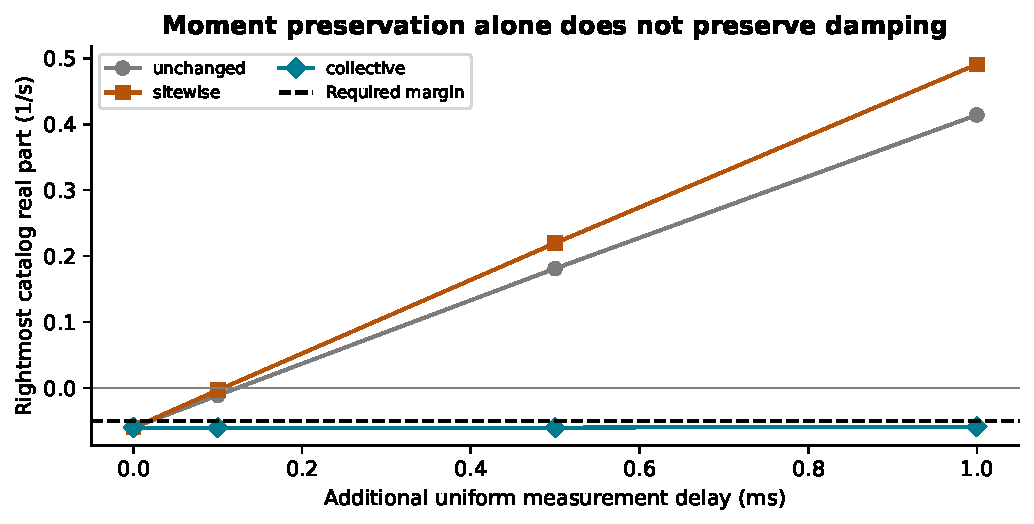
\includegraphics[width=.88\linewidth]{experiments/network_moment_codesign_20261004/FIG_02_DELAY_AND_DAMPING.pdf}
\caption{Exact-exponential pole calculations: equal moments do not protect
modal damping. Lines connect the declared samples, not a certified frontier.}\end{figure}
\begin{figure}[htbp]\centering
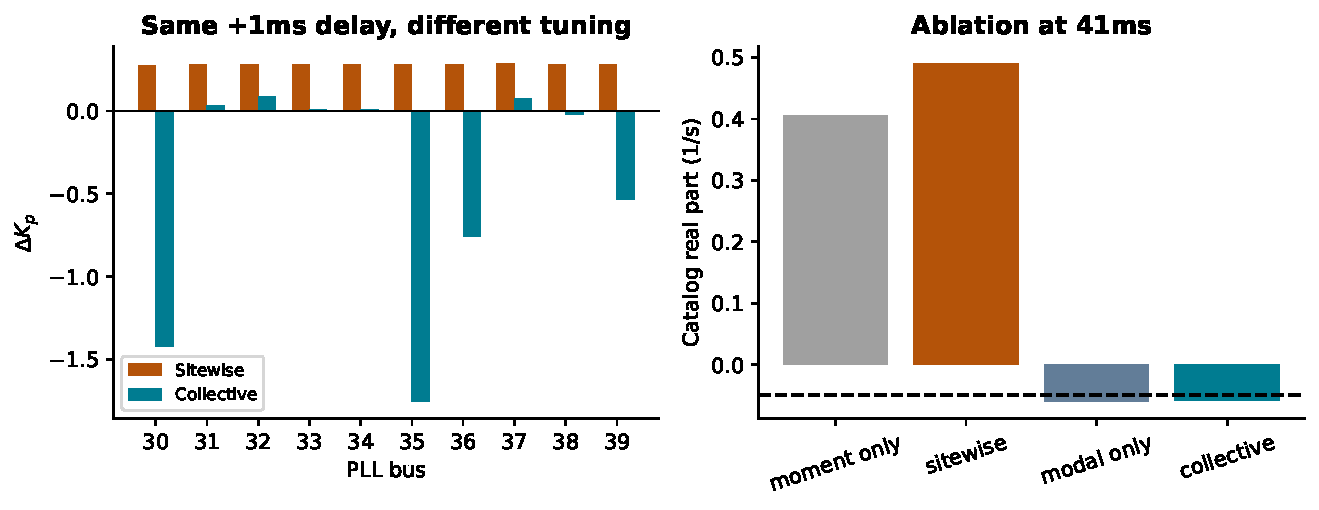
\includegraphics[width=\linewidth]{experiments/network_moment_codesign_20261004/FIG_03_TUNING_AND_ABLATION.pdf}
\caption{Finite tuning increments and algorithm ablations at 41 ms. Gain effort
is compared between local numerical candidates, not global optima.}\end{figure}
\begin{figure}[htbp]\centering
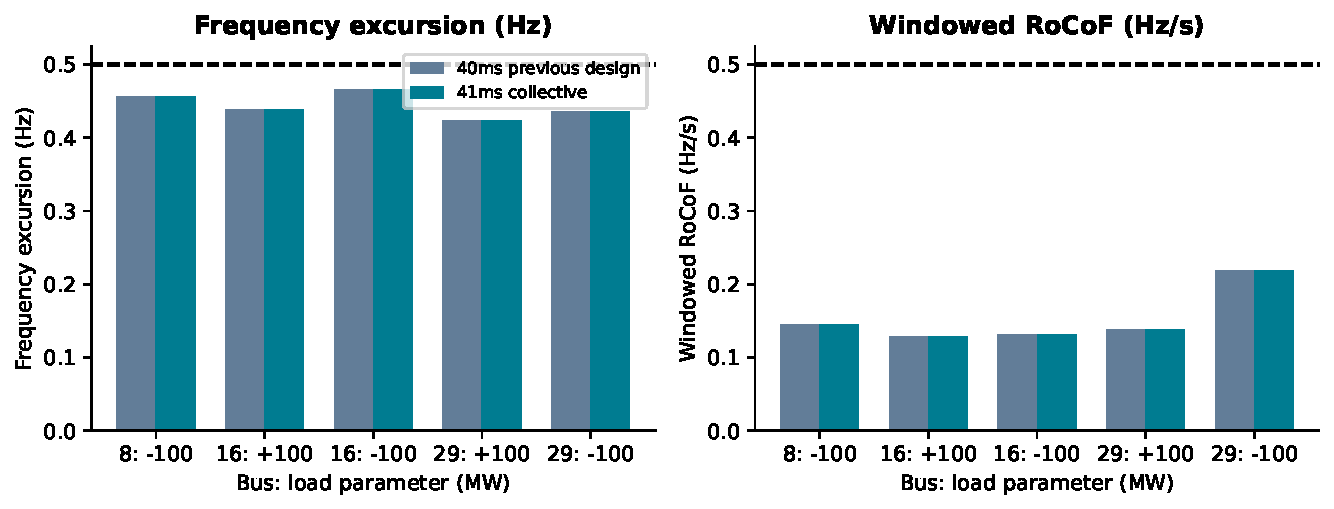
\includegraphics[width=\linewidth]{experiments/network_moment_codesign_20261004/FIG_05_NONLINEAR_EVENTS.pdf}
\caption{Five frozen nonlinear events. Frequency and RoCoF use the inherited
0.5 s window over all 39 bus voltage phases.}\end{figure}
